\section{Experimentación}

\subsection{Análisis de resultados para casos particulares}



Para ver como se comporta el algoritmo de $PageRank$ y comparar los resultados con los de $IN-DEG$, proponemos los siguientes ejemplos pequeños. Los grafos representan las páginas web y los link entre ellas, y las tablas muestran los resultados obtenidos de cada algoritmo.\\

\begin{figure}[H]
\centering     %%% not \center
\subfigure[Figure A]{\label{fig:a}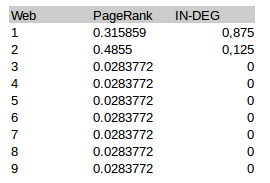
\includegraphics[width=0.4\linewidth]{imagenes/resultadosEstrella.png}}
\subfigure[Figure B]{\label{fig:b}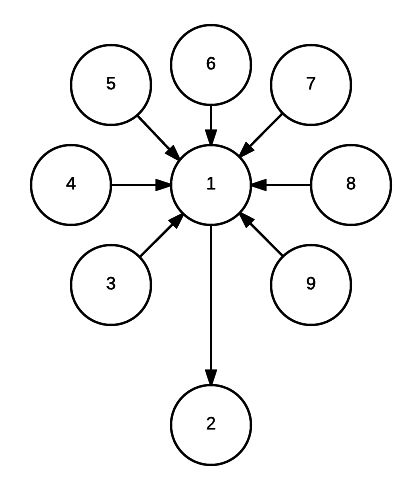
\includegraphics[width=0.3\linewidth]{imagenes/estrella.png}}
\caption{Web con estructura de estrella.}
\end{figure}

En el caso de una web con forma de estrella, cabe destacar las páginas 1 y 2. La página 1 es referenciada por todas las demás, salvo la 2 que es referenciada por la página 1. Dado que IN-DEG definie el ranking de una página j en base a la cantidad de ejes entrantes, es claro que la página uno obtenga la primer posición y la página 2 la segunda posición. Las páginas restantes tienen ranking cero por no ser referenciadas por ninguna otra.
En cambio, para PageRank se hace visible la idea de qué tan importante es el que referencia, en vez de cuantos son los que referencian. Las páginas que no son linkeadas tienen una importancia baja en comparación a las primeras dos.


\begin{figure}[H]
\centering     %%% not \center
\subfigure[Figure A]{\label{fig:a}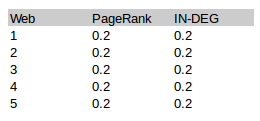
\includegraphics[width=0.4\linewidth]{imagenes/resultadosCompleto.png}}
\subfigure[Figure B]{\label{fig:b}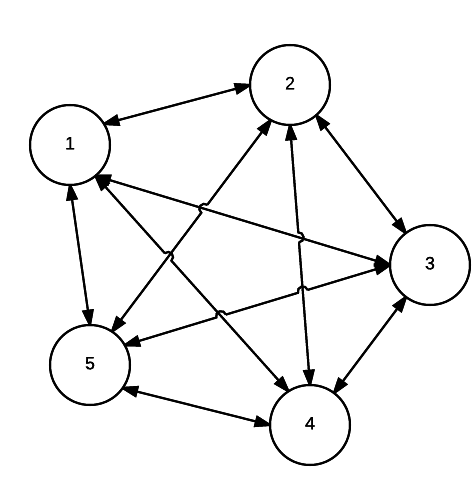
\includegraphics[width=0.3\linewidth]{imagenes/completo.png}}
\caption{Web con estructura de pentágono.}
\end{figure}

El segundo ejemplo, un grafo completo de cinco nodos, lo hicimos para encontrar los casos en que los criterios de importancia de ambos algoritmos coinciden. Era esperable que todas las páginas tengan la misma importancia en ambos dos, ya que todas las páginas web son referenciadas por páginas con la misma importancia.

\begin{figure}[H]
\centering     %%% not \center
\subfigure[Figure A]{\label{fig:a}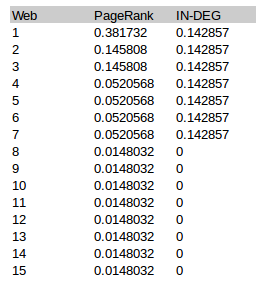
\includegraphics[width=0.3\linewidth]{imagenes/resultadosBinario.png}}
\subfigure[Figure B]{\label{fig:b}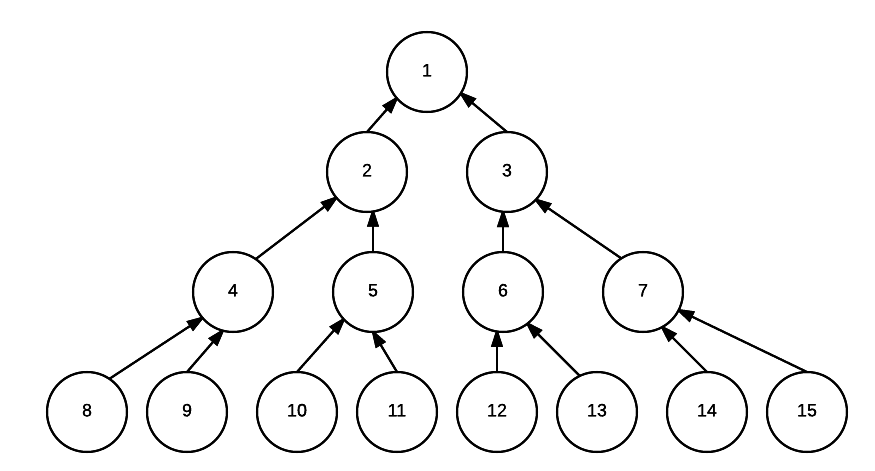
\includegraphics[width=0.5\linewidth]{imagenes/binario.png}}
\caption{Web con estructura de árbol binario.}
\end{figure}


\begin{figure}[H]
\centering     %%% not \center
\subfigure[Figure A]{\label{fig:a}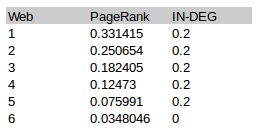
\includegraphics[width=0.4\linewidth]{imagenes/resultadosCamino.png}}
\subfigure[Figure B]{\label{fig:b}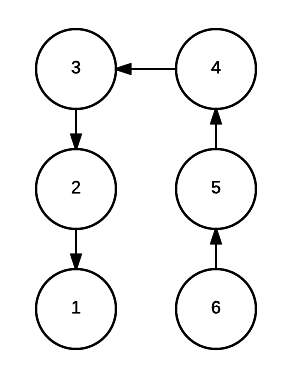
\includegraphics[width=0.2\linewidth]{imagenes/camino.png}}
\caption{Web con estructura de camino.}
\end{figure}

En los dos últimos graficos, se puede apreciar un comportamiento similar a los primeros dos, ya que la estructura subyacente a ambos es similar a las de estos 2 gráficos, generándose rankings similares.   



\begin{figure}[H]
\centering     %%% not \center
\subfigure[Figure A]{\label{fig:a}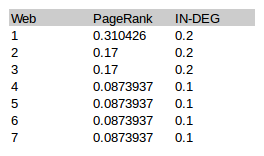
\includegraphics[width=0.4\linewidth]{imagenes/resultadosArbolRecursivo.png}}
\subfigure[Figure B]{\label{fig:b}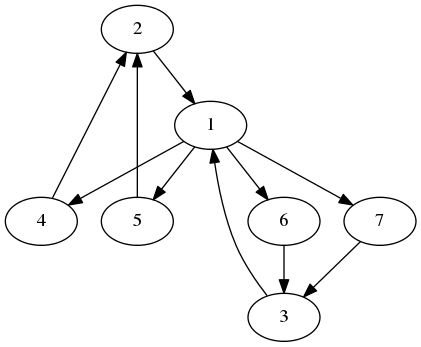
\includegraphics[width=0.4\linewidth]{imagenes/arbolRecursivo.png}}
\caption{Web con estructura de árbol recursivo.}
\end{figure}

Propusimos este último ejemplo porque suponíamos que el primer nodo iba a perder mucha importancia por contener links a los nodos más bajos del árbol. Pero esto no es tan asi: si bien el nodo uno disminuye su ranking y los nodos 4,5,6 y 7 aumentan su ranking, los resultados fueron similares al ejemplo del árbol binario. 

\newpage



\begin{wrapfigure}{r}{0.6\textwidth}
  \vspace{-20pt}
  \begin{center}
    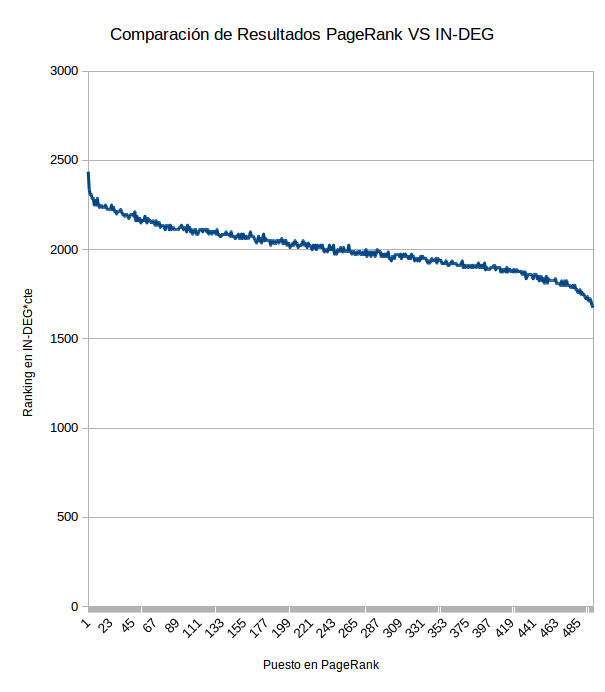
\includegraphics[scale= 0.6]{imagenes/pagerankVSindeg.png}
  \end{center}
  \vspace{-10pt}
  \vspace{-10pt}
\end{wrapfigure}

\subsection{Análisis de resultados}

Luego del análisis para casos chicos y particulares, para un análisis de resultados más general ejecutamos los algoritmos de $PageRank$ e $IN-DEG$ para una misma instancia de 500 páginas y 80000 links, con las webs de entrada y salida para cada link tomadas al azar entre las 500. Queremos ver cuánto cambian los rankings de cada web para cada algoritmo. Mientras que en el eje X está el puesto de las páginas según $PageRank$, en el eje Y está el valor del ranking de $IN-DEG$ para esa misma página (que está entre 0 y 1) multiplicado por una constante por cuestiones de claridad a la hora de visualizar el gráfico.\\


Podemos ver que en este caso particular, con una matriz bastante esparsa (30\% de los links aproximadamente), ambos algoritmos devuelven un resultado muy similar. Si los resultados fueran los mismos, deberíamos ver una linea recta en el gráfico. Lo que varía es el puesto en $PageRank$ de las webs que tienen pocos links entrantes de diferencia (varía mas en intervalos pequeños). \\


\subsection{Análisis de convergencia}
%Imagen 1
\begin{wrapfigure}{r}{0.6\textwidth}
  \vspace{-20pt}
  \begin{center}
    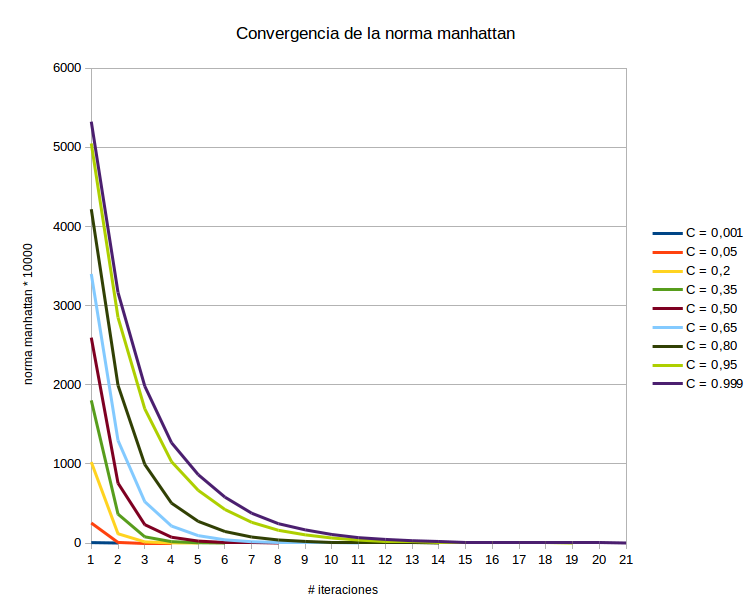
\includegraphics[scale= 0.6]{imagenes/convergencia1.png}
  \end{center}
  \vspace{-20pt}
   \caption{Con  1000 páginas y 3000 links.}
  \vspace{-10pt}
  \label{fig:img3}
\end{wrapfigure}

Para poder analizar la convergencia de $PageRank$ realizamos mediciones de la cantidad de iteraciones que hace el método de la potencia en el algoritmo, que termina cuando la norma de Manhattan es menor que un determinado valor de tolerancia. Tomamos como tolerancia el valor 0.00001 porque lo consideramos lo suficientemente chico.\\

Usamos tres instancias generadas al azar: La primera de 1000 páginas y 3000 links, la segunda de la misma cantidad de páginas pero 10000 links y la tercera de 500 páginas y 150000 links. Tomamos diferentes medidas de esparsidad, diferentes tamaños de matrices y diferentes valores de $c$ para ver que diferencias hay en la cantidad de iteraciones del método de la potencia.\\

Nos interesa ver qué hace que el algoritmo termine en una menor cantidad de pasos y qué relación hay entre ese número y el valor de $c$. Ejecutamos $PageRank$ para cada instancia con la tolerancia fija de 0,00001, variando el valor del $c$ desde 0,001 hasta 0,999. Cada gráfico corresponde a los resultados obtenidos para una instancia distinta.\\



%Imagen 2
\begin{figure}[h]
  \begin{center}
    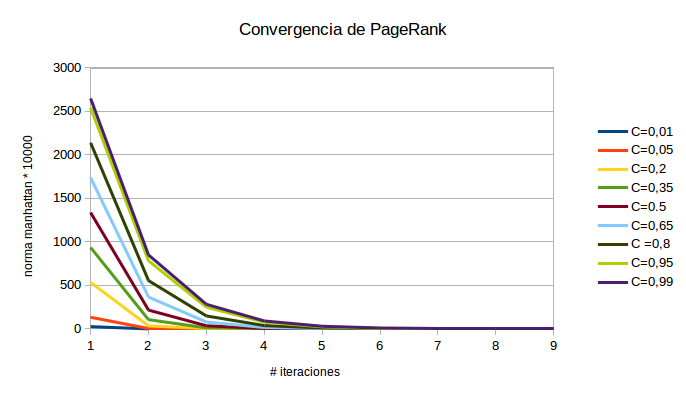
\includegraphics[scale= 0.6]{imagenes/convergencia2.png}
     \caption{Con 1000 páginas y 10000 links.}
  \end{center}
  \label{fig:img4}
\end{figure}



%Imagen 3
\begin{figure}[h]
  \vspace{-20pt}
  \begin{center}
    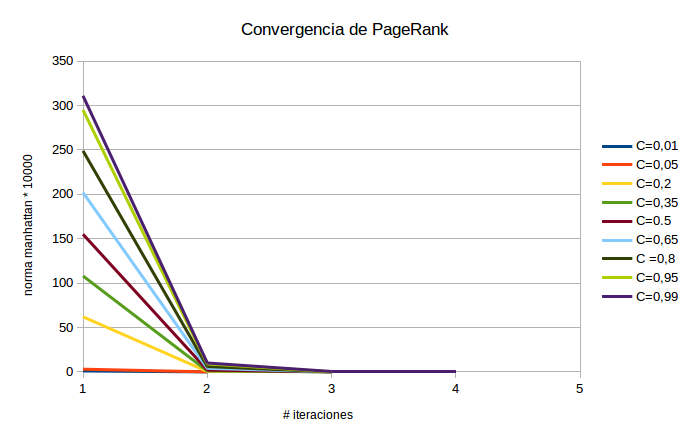
\includegraphics[scale= 0.6]{imagenes/convergencia3.png}
  \end{center}
   \caption{Con 500 páginas y 150000 links.}
  \label{fig:img5}
\end{figure}

Mirando cada gráfico por separado podemos ver que la cantidad de iteraciones del algoritmo disminuye mientras más chico sea el valor de $c$, independientemente de que tan esparsa sea la matriz de links. 
Además, si comparamos los tres gráficos, vemos que las normas son mas chicas y el algoritmo converge más rápidamente mientras mas completa (menos esparsa) sea la matriz de links. Más adelante vamos a ver si esto tambien influye en el tiempo de ejecución.\\

\newpage

\subsection{Análisis de performance}

Primero vamos a hacer un análisis de tiempos comparativo para cada estructura: Vector, DOK y CSR.

El siguiente grafico detalla los resultados temporales de haber corrido instancias para PageRank con las distintas estructuras de matriz. 

\begin{figure}[h]
   \begin{center}
     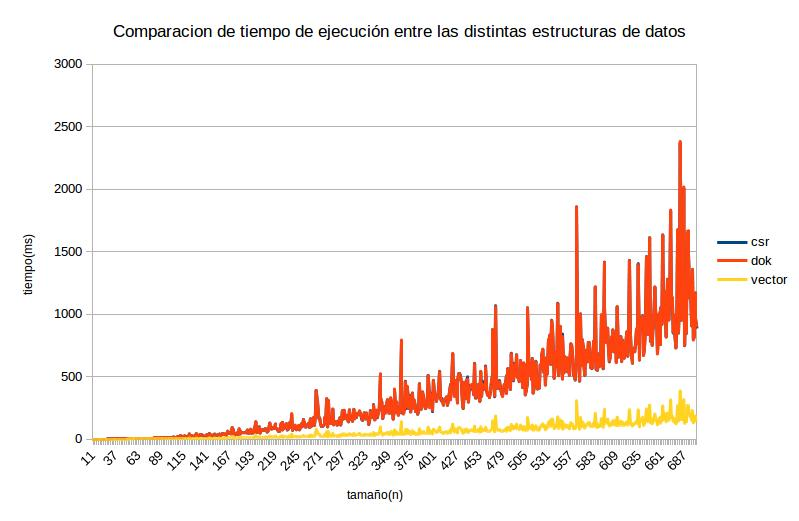
\includegraphics[scale=0.6]{imagenes/comparacion-tiempo-ejecucion-csr-dok-vector.png}
   \end{center}
   \caption{Gráfico que representa el tiempo de corrida de PageRank con distintas estructuras de datos.}
  \label{fig:img7}
\end{figure}

Pudimos observar que CSR fue el más rápido de los 3, ya que obtener los elementos y multiplicarlos es rápido, mientras que DOK es el más lento. A pesar de que tanto para CSR como DOK implementamos algoritmos más eficientes de multiplicación tanto para un escalar como para un vector, DOK resultó el más lento. \\

Creemos que esto se debe a la implementación interna de $map$ que está implementado sobre un Black-Red-tree. Tanto para multiplicar por un escalar como por un vector, iteramos por la estructura del mismo, de forma tal de aprovechar la esparcidad de la matriz y multiplicar sólo los elementos no nulos. En principio no encontramos una razón por la cual una implementación fuera mejor que la otra en cuanto a la forma de multiplicar desde el punto de vista algoritmico. Creemos que la razón radica en que, al iterar sobre los elementos de map se está haciendo una búsqueda binaria del próximo elemento en cada paso, dando como resultado que la complejidad de la operación no fuese $\mathcal{O}(nnz)$ sino $\mathcal{O}(nnz\log{}nnz)$ \\

Lo que nos resultó sorpresivo fue que incluso Vector tuvo una mejor performance que DOK, a pesar de que la complejidad de Vector para las operaciones anteriormente mencionadas es del orden cuadrático. Para este caso no pudimos obtener un resultado concluyente de por qué sucede esto. Una suposición a priori sugiere que se deba a optimizaciones realizadas por el compilador, explotando el hecho que Vector tenga todos sus elementos contiguos, disminuyendo así su tiempo de acceso. Sin embargo tal hipótesis excede nuestro análisis.\\

\newpage

El siguiente gráfico también mide le tiempo de ejecución para cada una de las estructuras pero en función de la esparcidad de la matriz, es decir, se usaron instancias con matrices de tamaño fijo $140x140$ y se fue incrementando la cantidad de links desde 4 hasta 19384 haciéndola cada vez menos esparsa. Cada instancia tiene distribuidos los links de forma aleatoria. Queremos ver qué sucede con el tiempo de ejecución cuando se varía unicamente la esparsidad de la matriz. \\

\begin{wrapfigure}{r}{0.6\textwidth}
  \vspace{-20pt}
  \begin{center}
    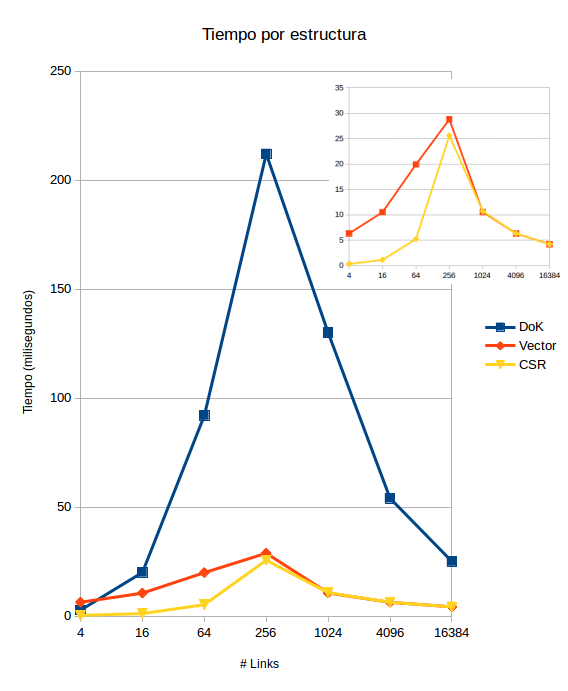
\includegraphics[scale=0.4]{imagenes/MedicionTiempoEstructura.png}
  \end{center}
  \vspace{-20pt}
  \vspace{-10pt}
  \label{fig:img8}
\end{wrapfigure}

Vemos que para la estructura de CSR el tiempo es menor que el de la estructura vector para matrices muy esparsas, pero el tiempo para ambas estructuras es muy parecido cuando la matriz es poco esparsa. En cambio, cuando usamos la estructura de DOK, el tiempo dió mucho mayor para todas las instancias de matrices esparsas que generamos. Esto se debe, como dijimos anteriormente, a otros aspectos que no tienen que ver con la esparsidad de la matriz. Recordemos que en el contexto de aplicación las matrices van a ser en general muy esparsas (hay pocos links entre las páginas web en comparación con el máximo que podría haber), motivo por el cuál en este caso es más rápido usar CSR.\\ 

Por otro lado, en un punto vemos que el tiempo comienza a disminuir. Esto tiene que ver con la cantidad de iteraciones que realiza el algoritmo del método de la potencia. Como vimos en los experimentos en los que analizamos la convergencia, mientras menos esparsa es la matriz, el método de la potencia realiza menos iteraciones y termina de ejecutar más rápidamente. \\

Realizamos otro experimento utilizando una intancia grande de un conjunto de páginas web reales y los links entre ellas. Las páginas web son de Stanford y las cantidades de páginas y links son 281903 y 2312497. La matriz de links es muy esparsa. Medimos los tiempos de ejecución para esta instancia utilizando las distintas estructuras. Como era previsto, el tiempo de ejecución con CSR fue mucho menor, seguido por el tiempo de DOK y el tiempo de Vector, de manera ascendente.

Ahora vamos a hacer un análisis temporal de $PageRank$ en función únicamente de la cantidad de páginas, utilizando la estructura elegida CSR.

Generamos instancias con una cantidad determinada y ascendente de nodos desde 100 hasta 800. Todas las instancias tienen un mismo nivel de esparcidad del 30 por ciento de la cantidad máxima de links posibles. De esta manera vemos que relación hay entre el tiempo de ejecución y el tamaño de la matriz. \\

Los siguientes gráficos muestran los tiempos obtenido. El primero muestra el tiempo real y el segundo muestra los tiempos de los mismos experimentos pero divididos por la cantidad de nodos al cuadrado del grafo de cada instancia.\\

\newpage

\begin{figure}[h]
   \begin{center}
    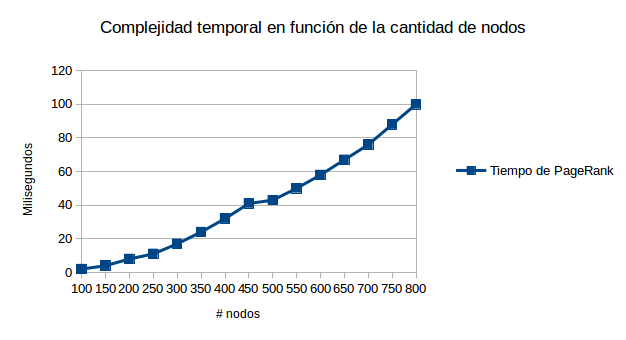
\includegraphics[scale= 0.8]{imagenes/complejidadcuadratica.png}
   \end{center}
   \caption{Gráfico que representa el tiempo de corrida de PageRank}
  \label{fig:cuad}
\end{figure}

\begin{figure}[h]
   \begin{center}
     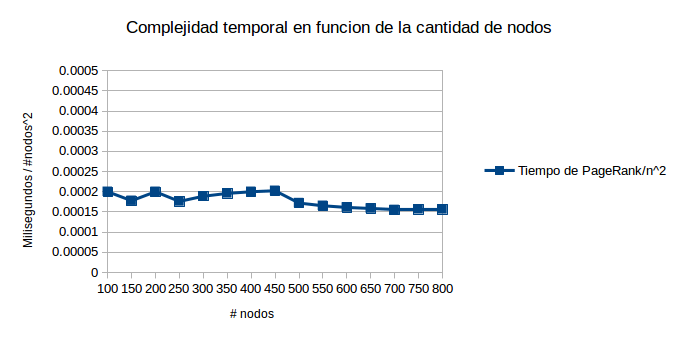
\includegraphics[scale= 0.8]{imagenes/complejidadlineal.png}
   \end{center}
   \caption{Gráfico que representa el tiempo de corrida de PageRank dividido por el tamaño al cuadrado}
  \label{fig:lin}
\end{figure}

 Podemos ver de esta manera que la complejidad del algoritmo es cuadrática con respecto al tamaño de la matriz, ya que el segundo gráfico es constante. \\

Si bien el tiempo de CSR se ve disminuido porque las matrices son esparsas, la complejidad es la misma si se usa alguna de las otras estructuras que vimos, ya que sólo cambia en una constante (depende de la esparsidad) multiplicativa. \\

\newpage

\subsection{Análisis de resultados de GeM y el método alternativo para ligas deportivas}

Para analizar los resultados de GeM y nuestro método alternativo, utilizamos los resultados reales de un torneo de fútbol (Torneo Final 2014 Argentina). Son 20 equipos, y cada uno de ellos juega una única vez con cada uno de los otros, a lo largo de 19 fechas de enfrentamientos. Los demás parámetros para ejecutar esta instancia fueron: 0.65 de probabilidad de teletransportación, 0.00001 de tolerancia para el método de la potencia. Más adelante analizaremos que sucede con los rankings cuando se varía la probabilidad de teletransportación.

En este caso, para cada equipo analizamos la posición en que quedaron en la última de las fechas con los dos algoritmos y las posiciones finales reales. En el siguiente gráfico vemos como variaron las posiciones. 


\begin{figure}[H]
  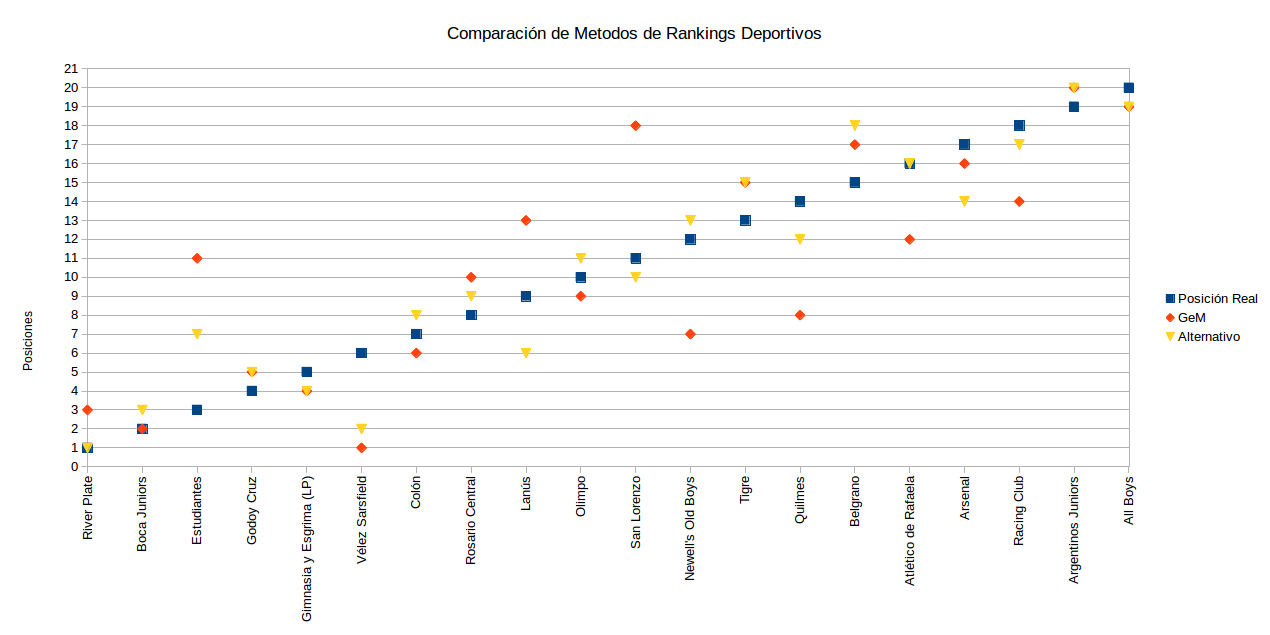
\includegraphics[scale=0.5]{imagenes/posicionesgem.png}
   \caption{Gráfico que compara las posiciones reales y las obtenidas con GeM y nuestro método alternativo.}
  \label{fig:img1}
\end{figure}

Las posiciones resultantes de nuestro método alternativo se asemejaron más a las posiciones reales, ya que ambos métodos de ranking utilizan la información de si se gana o no un partido y con cuántos goles. El método de GeM también tiene en cuenta el ranking del equipo contra el que se enfrentó. De manera que el impacto en el ranking de un equipo en una fecha depende del resultado de todos los partidos de esa fecha.

%%%%%%%%%%%%%ANALIZAR lOS PICOS
Primero, analizamos el impacto de los empates en GeM y otros casos de interés para luego analizar los datos obtenidos de los datos reales. Dado un empate, no se le suma nigun valor a la posición correspondientes de los equipos en la matriz que representa los resultados. Lo mismo sucede en caso de que un equipo pierda contra otro. Al equipo perdedor, no se le suma valor. De esta forma, lo que queda plasmado es que un empate, en GeM, tiene el mismo efecto que haber perdido (salvo por el beneficio hacia el equipo ganador). \\ \\
Realizamos un pequeño experimento con tres equipos A, B y C, donde A siempre empataba contra los otros dos, y B le ganaba siempre a C. El resultado obtenido es que tanto A como C tienen el mismo ranking, sin importar cuantos partidos jueguen cada uno (siempre manteniendo el invariante anterior), ni tampoco por cuanta diferencia de goles gana B. Luego lo modificamos, de forma que en lugar de empatar, A gane un partido contra B y contra C, pierda un partido contra B y C (por la misma diferencia), y B le siga ganando siempre a C. La idea era ver que sucedia si se mantenia este equilibrio en A de ganar y perder, y si impactaría en el resultado final. Obtuvimos que los resultados era exactamente iguales al caso anterior, donde A y C tienen el mismo ranking, mientras que el de B es superior. Aumentamos el numero de vece que gana B y también su diferencia y no importa cuantas veces gane B ni por cuanto, esto no altera la posicion de C. \\
La razón de este resultado es que, en ambos casos, las columnas de A y C tienen los mismos valores, por tal motivo se obtiene el mismo ranking. Cabe destacar que para el primer caso, para el método real, si se empata y pierde se obtiene un solo punto, mientras que si se empata dos veces se obtienen dos puntos, no siendo los resultados finales iguales. Aquí vemos un caso claro de diferencia entre ambos métodos. \\
También, quisimos ver el impacto de las diferencias de goles. Corrimos una instancia donde A y B le ganan a C, donde A le gana por mucha más diferencia que B. Nuestras hipótesis eran que, o A y B iban a tener el mismo ranking y C uno más bajo, o que A tendría un rakning más alto que B, y B más alto que C. Observamos que sucedía lo segundo, por lo que disminuimos la diferencia de goles de A y C, de forma de acercarse al de B (pero superandolo), y observamos que sus rankings diferían menos. Por lo tanto, la diferencia de goles es un factor que impacta directamente en el resultado de GeM. \\
Por último, nos planteamos las siguiente pregunta: ¿Es mejor ganar por poco muchas veces, o ganar por mucho pocas veces? Suponiendo que el resto de las variables se mantienen igual, no habría diferencia en tanto la suma de las diferencias sea la misma porque se obtiene el mismo resultado en la matriz que usamos.
\\
Ahora veamos como varían las posiciones obtenidas con GeM para algunos equipos a lo largo de ese mismo campeonato (fecha a fecha). Los resultados de cada fecha incluyen todos los partidos jugados hasta dicha fecha (incluidas todas las fechas anteriores).
Elegimos analizar los rankings solamente de aquellos equipos que nos resultó interesante estudiar en detalle.

\begin{figure}[H]
  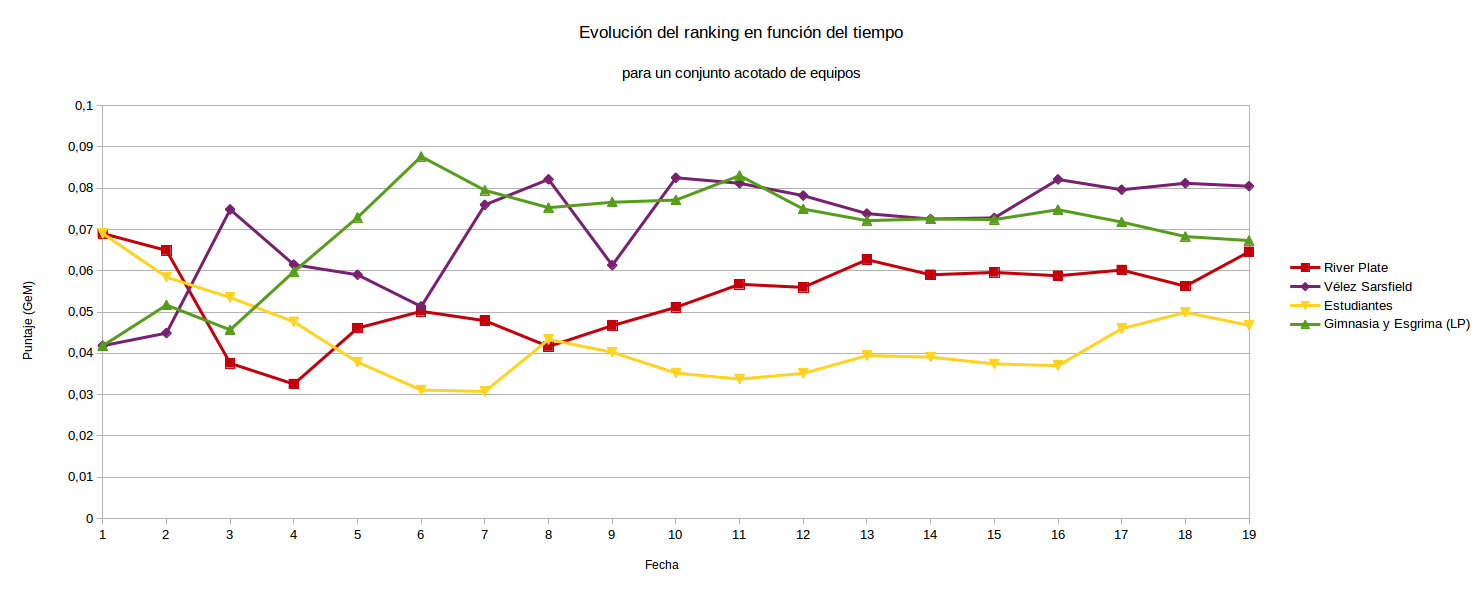
\includegraphics[scale=0.449]{imagenes/gemfechas2.png}
   \caption{Gráfico que muestra los resultados de GeM fecha a fecha para algunos equipos.}
  \label{fig:img1}
\end{figure}

Vemos que los rankings de estos equipos varían mucho en las primeras fechas, pero a medida que transcurre el campeonato tienden a estabilizarse. Esto es porque la información nueva obtenida impacta de forma menos considerable en el resultado acumulado.\\

Los equipos que elegimos para analizar son: el ganador en el ranking real (River Plate), el ganador en el ranking de GeM (Vélez Sarsfield), el equipo con variación máxima entre el ranking real y el ranking de GeM (Estudiantes), y otro equipo que nos llevó a resultados interesantes el comportamiento de GeM (Gimnasia y Esgrima).\\

Primero, analizaremos el caso de Gimnasia y Esgrima. Como se ve en el gráfico, tiene un gran crecimineto entre las fechas 3 y 6. En principio creíamos que era poque había ganado todos los partidos durante ese tiempo. Sin embargo esto no resulta ser así. En la fecha 4 empató, en la 5 ganó y en la 6 volvió a empatar. A pesar de esto, su ranking creció constantemente. Esto se debe a que en la fecha 2 le ganó a Newell's Old Boys 3 a 0. Además, Newell's Old Boys ganó dos partidos por una diferencia de 3 goles, y los otros dos partidos los empató. Por esta razón, creemos que Gimnasia y Esgrima crece en su ranking dado que le ganó a un equipo en fechas anteriores que en las subsiguientes fechas ganó por mucho. \\

Nos resultó muy dificultoso realizar un análisis detallado de por qué saldría campeón Vélez Sarsfield utilizando el método GeM en lugar de River Plate como sucede en el ranking oficial. El dato más destacable de la fecha que puede impactar en este resultado, es que Vélez Sarsfield hizo 34 goles y fue el equipo que más goles hizo durante todo el campeonato, seguido de River Plate con 28, aunque no pudimos encontrar una relación entre esta información y los resultados obtenidos con GeM. La baja en el puntaje de River Plate se ve principalmente en las fechas 2, 3 y 4, dónde empata la primera y pierde las dos siguientes, momento a partir del cual empieza a subir su puntaje, pero no lo suficiente como para superar a Vélez Sarsfield. Por otro lado, Vélez aumenta considerablemente su posición en la fecha 7 donde le gana 3 a 1 a Belgrano, y en al fecha 10 le gana 5 a 1 a Gimnasia y Esgrima, momento a partir del cual su puntaje se estabiliza. Al haber ganado estos últimos partidos por una diferencia considerable, se ve favorecido en el método GeM. Creímos que la diferencia en los resultados radica en la suma de la diferencia de goles positiva (osea solo las diferencias donde un equipo gana) porque son los datos que se ven plasmados en la matriz de GeM. Sin ambrgo, la suma de las diferencias positivas es 18 para ambos equipos, por lo que concluimos que la diferencia está en a qué equipos le gana Velez Sarfield para salir Campeón. Analizamos este aspecto, pero tampoco pudimos obtener resultados concluyentes. Sumamos los rankings finales de los equipos a los que le ganó Velez, obtenienndose 0.436 y a los que le ganó River, siendo 0.559. Aquí tampoco vemos los resultados esperados, ya que supusimos que Vélez obtendría una suma mayor por haber ganado a equipos con mayor ranking. El único resultado que apunta en esta dirección es que, de las 9 victorias de Vélez, 5 fueron contra equipos entre los primeros 10, y de las 11 victorias de River, 7 son contra equipos en las últimas 10 posciones. \\

Por último, para el caso de Estudiantes, el cual se ubica en la tercera posición en el ranking oficial.  A pesar de haber ganado 3 veces hasta la fecha 7, su ranking desciende constantemente. Esto se debe a que gana contra equipos que tienen ranking bajo, y empata o pierde contra equipos de mayor ranking. En la fecha 8, le gana a Gimnasia y Esgrima, que en ese momento es el equipo con mayor puntaje, favoreciendolo significativamente. Luego, no gana partidos contra equipos de mucho ranking, lo que no le permite crecer significativamente. La razón de la diferencia de posiciones radica en que, a pesar de ser el tercer equipo con mayor cantidad de victorias, estas victorias fueron contra equipos que no tienen tanto peso en el ranking, por lo tanto en el método GeM se ve perjudicado. \\
\\

Como conclusión, vemos que realizar un análisis de GeM no es sencillo dado que no sólo impacta los resultados de un equipo en particular en cada fecha, sino que todos los resultados impactan en el resultado de todos los demás, aún no habiendo jugado en contra. En el caso de los empates, el método de GeM no los considera pero igualmente un equipo puede ascender o descender en su posición por los resultados del resto de los partidos de la fecha. Sucede lo mismo aún habiendo ganado o perdido, por ejemplo en la fecha 12 donde Gimnasia y Esgrima le ganó a Olimpo y bajó su ranking, o en la fecha 8 donde Vélez Sarfield pierde contra Atlético de Rafaela e igualmente sube su posición. Sin embargo, se tiene un método donde ganar o perder contra uno u otro equipo no tiene el mismo peso que en el método oficial.


\subsection{Análisis de resultados variando la probabilidad de teletransportación en $PageRank$}

Utilizamos los resultados del Torneo Final 2014 Argentina de la sección anterior. Ejecutamos el algoritmo de $GeM$ para conseguir la tabla de posiciones, variando el valor del parámetro $c$ desde 0.1 hasta 0,99. El siguiente gráfico muestra para cada equipo, el ranking obtenido.\\

\begin{figure}[H]
\centering
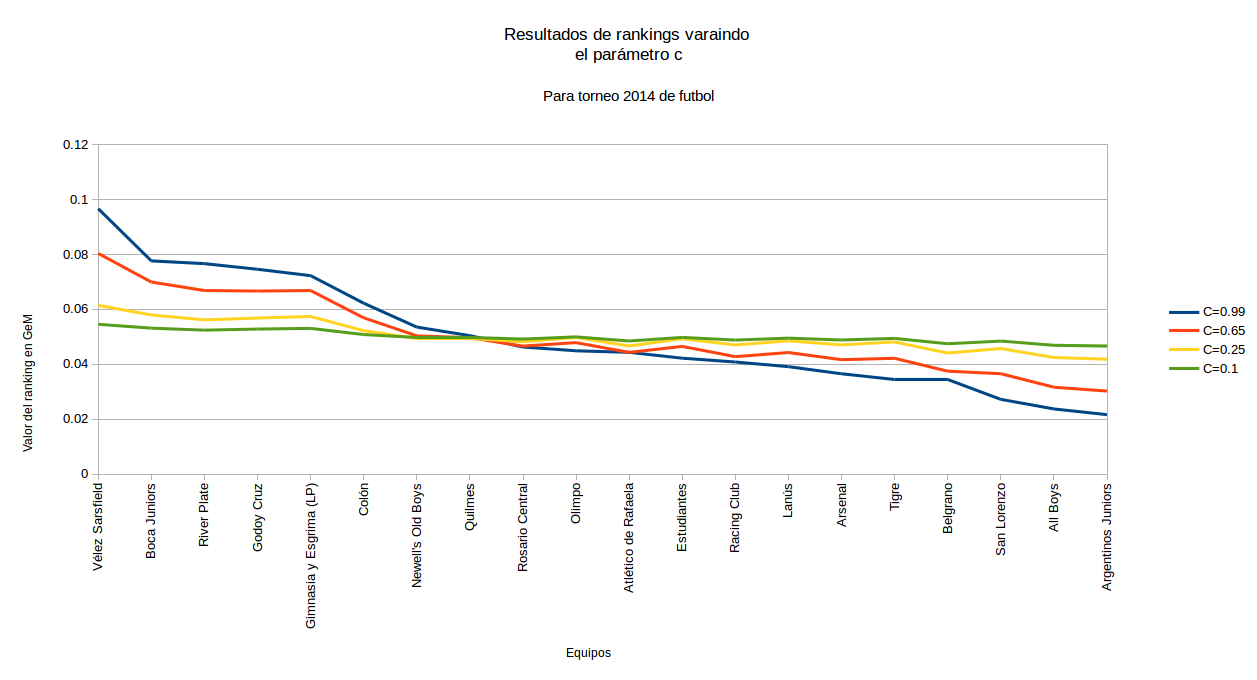
\includegraphics[width=0.7\linewidth]{imagenes/varicionCfutbol2014Ordenado.png}
\end{figure}

Los equipos están ordenados de mayor a menor (de derecha a izquierda) de a cuerdo al resultado obtenido con el $c$ de mayor valor. Vemos que al disminuir el $c$, lo que sucede es que las posiciones tienden a variar menos, achatandose el gráfico de los resultados obtenidos.
Por este motivo, un valor de $c$ distinto puede variar el puesto de los equipos que tengan un ranking cercano. Por ejemplo, para $c=0.1$, River Plate saldría quinto, mientras que con $c=0.99$, saldría tercero. Sin embargo, en general, se mantiene una tendencia del orden de los equipos. 
